% !TEX root = ./Vorlesungsmitschrift DIFF 2.tex  
\lecture{Mo 04.05. 10:15}{}
\section{Stetige Abbildungen in normierten Vektorräumen}
\subsection{Lineare Abbildungen}
\begin{satz}\label{lineare_abbildung:stetigkeitssatz}
    Seien \( (V,\norm{\cdot}_{V}) \) und \( (W,\norm{\cdot}_{W}) \) normierte Vektorräume.
    Sei \( A\maps V\to W \) linear.
    Dann sind folgende Aussagen äquivalent:
    \begin{eigenschaftenenumerate}
        \item \label{lineare_abbildung:stetigkeitssatz:stetig} \( A \) ist stetig
        \item \label{lineare_abbildung:stetigkeitssatz:stetig_in_null} \( A \) ist stetig in \( 0 \)
        \item \label{lineare_abbildung:stetigkeitssatz:norm_beschraenkt} \( \norm{A(x)}_{W}\leq C\norm{x}_{V} \).
    \end{eigenschaftenenumerate}
    
\end{satz}
\begin{proof}
    \begin{proofdescription}
        \item[\ref{lineare_abbildung:stetigkeitssatz:stetig} \timplies \ref{lineare_abbildung:stetigkeitssatz:stetig_in_null}] \checkmark
        \item[\ref{lineare_abbildung:stetigkeitssatz:stetig_in_null} \timplies \ref{lineare_abbildung:stetigkeitssatz:norm_beschraenkt}] \( A \) stetig in \( 0 \) \timplies zu \( \varepsilon=1 \) \texists \( \delta>0 \) \sd
        \begin{align*}
            \norm{A(y)-A(0)}_{W}\overset{\text{Lin}}{=}\norm{A(y)}_{W}<1\quad \forall y\in V \text{ mit }\norm{y-0}_{V}=\norm{Y}_V<\delta.
        \end{align*} 
        Setze \( C\definedas \quot{2}{\delta} \).
        Sei \( x\in V\setminus \zeroset \) beliebig (für \( x=0 \) gilt die Ungleichung \ref{lineare_abbildung:stetigkeitssatz:norm_beschraenkt} ohnehin).
        Setze \( \lambda\definedas \quot{1}{C\norm{x}_{V}} \) und \( y\definedas \lambda x \).
        
        Dann ist \( \norm{y}_V=\frac{1}{C\norm{x}_V}\norm{x}_V=\quot{\delta}{2}<\delta \), also \( \norm{A(y)}_W<1 \).
        \begin{align*}
            A(y)=A(\lambda x)=\frac{1}{C\norm{x}_V}A(x)\implies \Beh.
        \end{align*}
        \item[\ref{lineare_abbildung:stetigkeitssatz:norm_beschraenkt}\timplies \ref{lineare_abbildung:stetigkeitssatz:stetig}] Es gebe \( C>0 \) \sd
        \begin{align*}
            \norm{A(x)}_{W}\leq C\norm{x}_V \quad \forall x\in V.
        \end{align*} 
        Dann gilt insbesondere für \( x=y-a \).
        \begin{align*}
            \norm{A(x)}_{W}\explain{\text{Linearität}}{=}\norm{A(y)-A(a)}\leq C\norm{y-a}_{V}.
        \end{align*}
        Sei \( \varepsilon>0 \).
        Dann ist also
        \begin{align*}
            \norm{A(y)-A(a)}_{W}<\varepsilon\quad \forall y,a \text{ mit }\norm{y-a}_{V}<\frac{\varepsilon}{C}
        \end{align*}
        und somit ist \( A \) sogar gleichmäßig stetig.
    \end{proofdescription}    
\end{proof}
\begin{beispiele*}
    \begin{enumerate}
        \item \( (\stetigefunktionen(\interval{a}{b},\reals),\supnorm{\cdot}) \).
        \begin{align*}
            I\maps \stetigefunktionen(\interval{a}{b})\to \reals,\logicspace I(f)\definedas \Integrate{f(t)}{t,a,b}.
        \end{align*}
        \( I \) ist linear und es gilt
        \begin{align*}
            \norm{I(f)}\leq (b-a)\supnorm{f}
        \end{align*}
        \timplies \( I \) ist stetig.
        \item \( \totalderivative+;\maps (\stetigefunktionen^1(\interval{a}{b}),\supnorm{\cdot})\to (\stetigefunktionen(\interval{a}{b}),\supnorm{\cdot}) \), \( \totalderivative+;\maps f\mapsto f' \).
        \begin{behauptung*}
            \( \totalderivative+; \) ist nicht stetig.
        \end{behauptung*}
        \begin{proof}[Denn:]
            \( D \) ist linear \checkmark, aber die Bedingung aus \thref{lineare_abbildung:stetigkeitssatz} ist verletzt: Betrachte \( f_n\in C^1(\interval{0}{2}) \), \( f_n=x^n    \).
            Dann ist \( \supnorm{f_n}=1 \), aber \( \supnorm{\totalderivative{f_n}}=n \) \timplies es kann kein \( C>0 \) geben \sd
            \begin{align*}
                n=\supnorm{\totalderivative{f_n}}\leq C\norm{f_n}=C\quad \forall n.
            \end{align*}
        \end{proof}
    \end{enumerate}
\end{beispiele*}
\begin{definition*}\index{Operatornorm}
    Seien \( V \) und \( W \) normierte Vektorräume.
    Sei \( A\maps V\to W \) lineare stetige Abbildung.
    Die \emph{Operatornorm} von \( A \) ist definiert als
    \begin{align*}
        \norm{A}_{\text{op}}\definedas \sup_{\substack{x\in V\\ x\neq 0}}\frac{\norm{Ax}_{w}}{\norm{x}_{V}}.
    \end{align*}
\end{definition*}
    Auf dem VR der stetigen linearen Funktionen \( V\to W \) ist \( \norm{\cdot}_{\text{op}} \) eine Norm.
    \( \norm{A}_{\text{op}} \) ist die kleinste Konstante für die noch die Abschätzunge aus \ref{lineare_abbildung:stetigkeitssatz} gilt und es folgt
\begin{bemerkung}
    Ein linearer Operator ist genau dann stetig, wenn gilt \( \norm{A}_{\text{op}}<\infty \).
\end{bemerkung}
\begin{beispiel*}
    Ist \( A\maps \reals^n \to \reals^m \) linear, so gilt 
    \begin{align*}
        A\in \Mat(m\times n,\reals)\simeq \reals^{m\cdot n}.
    \end{align*}
    Daher ist \( \norm{\cdot}_{\text{op}} \) in diesem Fall äquivalent zu in \( \supnorm{\cdot} \), \( \supnorm{A}=\max_{i,j}\abs{A_{ij}}<\infty \), insbesondere also schwächer und somit ist \( A \) stetig.

    Konkret gilt: Setze \( V=(\reals^n, \norm{\cdot}_{V}) \), \( W=(\reals^n,\norm{\cdot}_W) \).
    Sei \( y=Ax \) \timplies \( y_i=\sum_{j=1}^{n}A_{ij}x_j\) für \( i=1,\dotsc,m \).
    \begin{align*}
        &\norm{y}_{W}\begin{aligned}[t]
            &\overset{\triangle}{\leq}\sum_{i=1}^{m}\norm{y_i e_i}_{W}\\
            &\stackrel[\mathclap{\text{Hom}}]{\triangle}{\leq}\sum_{i,j}\abs{A_{ij}x_j}\norm{e_i}_{W}\\
            &=\sum_{i,j}\abs{A_{ij}}\cdot\abs{x_k}\cdot\norm{e_i}_{W}\\
            &\leq \supnorm{A}\cdot\norm{x}_{\ell^1}\cdot \underbrace{\sum_{i=1}^{m}\norm{e_i}_W}_{=c_W}
        \end{aligned}\\
        \implies &\norm{A}_{\text{op}}=\sup_{x\neq 0}\frac{\norm{Ax}_{W}}{\norm{x}_V}\leq \supnorm{A}\cdot C_W\cdot\underbrace{\sup_{x\neq 0}\frac{\norm{x}_{\ell^1}}{\norm{x}_V}},        
    \end{align*}
    wobei \( C_V \) eine Konstante ist mit
    \begin{align*}
        \norm{x}_{\ell^1}\leq C_V\cdot \norm{x}_V\quad \forall x\in V=\reals^n.
    \end{align*}
\end{beispiel*}
\begin{bemerkung*}
    Unsere Beschränkung auf den \( \reals^n \) (statt beliebige endlich-dimensionale Vektorräume zuzulassen), bedeutet also keine Einschränkung, da ein Basiswechsel nach der Überlegung oben stetig ist.
\end{bemerkung*}
\begin{beispiele}
    \( f\maps \reals^n\to \reals^m \).
    \begin{eigenschaftenenumerate}
        \item \emph{Kurven} \( \gamma\maps I\to \reals^n \), \( I \) Intervall, stetig.
        \begin{beispiele*}
            \item \( \gamma\maps \interval{0}{2\pi}\to \reals^2 \), \( t\mapsto (r \Cos{t}, r \Sin{t}) \), \( r>0 \).
            Stetigkeit: Wir versehen \( \reals^2 \) mit \( \supnorm{\cdot} \).
            Dann folgt die Stetigkeit von \( \gamma \) aus der Stetigkeit der Komponentenfunktionen \( I\to \reals \).
            \item \( \gamma\maps \reals\to \reals^2 \), \( t\mapsto (t^2-1,t^3-1) \) genauso.
            Spur von \( \gamma=\Set{\gamma(t)|t\in \reals} \)
            \begin{figure}[H]
                \centering
                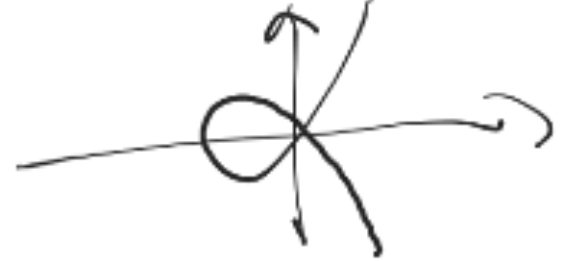
\includegraphics[width=0.5\linewidth]{figures/komponentenstetigkeit_beispiel_hoch_2_gegen_hoch_3}
                \label{fig:komponentenstetigkeit_beispiel_hoch_2_gegen_hoch_3}
            \end{figure}
        \end{beispiele*}
        \item\label{stetigkeit:beispiel:gebrochen_rationale_funktionen} Gebrochen rationale Funktionen:
        \begin{beispiele*}
            \item \( f\maps \reals^2\to \reals \).
            \begin{align*}
                f(x,y)=\begin{cases}
                    \frac{x^2y}{x^2+^2}&(x,y)\neq (0,0)\\
                    0&(x,y)=(0,0).
                \end{cases}                
            \end{align*}
            \( f \) ist stetig: auf \( \reals^2\setminus \zeroset \) sicherlich als Verknüpfung und Produkt stetiger Funktionen:
            \begin{align*}
                f=\text{Inv}\circ p_1\cdot p_2\quad \text{Inv}(t)=\frac{1}{t},\quad p_1(x,y)=x^2+y^2,\quad p_2(x,y)=x^2y.
            \end{align*}
            Stetigkeit in \( 0 \): Es gilt \( (x-y)^2\geq 0 \)
            \begin{align*}
                \implies &2\abs{xy}\leq x^2+y^2\\
                \implies &\abs{\frac{x^2y}{x^2+y^2}}<\frac{\abs{x}}{2}
            \intertext{für \( ((x_n,y_n))_{n} \), \( (x_n,y_n)\goesto(0,0) \) (bezüglich irgendeiner Norm) gilt insbesondere \( x_n\goesto 0 \)}
                \implies &\abs{f(x_n,y_n)-0}=\abs{\frac{x_n^2 y_n}{x_n^2+y_n^2}}<\frac{\abs{x_n}}{2}\goesto 0 \logicspace \text{in }\reals.
            \end{align*}
            \item \( f\maps \reals^2\to \reals \),
            \begin{align*}
                f(x,y)=\begin{cases}
                    \frac{x^2y}{x^4+y^2}&(x,y)\neq (0,0)\\
                    0&(x,y)=(0,0).
                \end{cases}
            \end{align*}
            \( f \) ist stetig auf \( \reals^2\setminus \zeroset \) (siehe oben).
            \( f \) ist nicht stetig in \( 0 \): Betrachte etwa \( (x_n,y-n)=\p*{ \frac{1}{n}, \frac{1}{n^2} } \), \( n\geq 1 \).
            Dann gilt
            \begin{align*}
                f(x_n,y_n)=\frac{1}{n^2n^2}\p*{ \frac{n^4}{2} }=\frac{1}{2}\cancel{\goesto}0.
            \end{align*}
            \minisec{Achtung:}
            Es gibt durchaus Folgen \( (x_n,y_n)\goesto 0 \) \sd \( f(x_n,y_n)\goesto 0 \) (für \( n\goesto \infty \)), \zb \( (x_n,y_n)=\p*{ 0,\frac{1}{n} } \), wo \( f\p*{ 0,\frac{1}{n} }=0\quad \forall n \) oder \( (x_n,y_n)=\p*{ \quot{1}{n},\quot{1}{n} } \) wo 
            \begin{align*}
                f(x_n,y_n)=\frac{1}{n^2}\p*{ \frac{n^2}{1+\quot{1}{n^2}} }\goesto 0.
            \end{align*}

            Daher muss man, wenn man Stetigkeit zeigen will, in Argument finden, dass für \emph{alle} Folgen funktioniert.
            \begin{figure}[H]
                \centering
                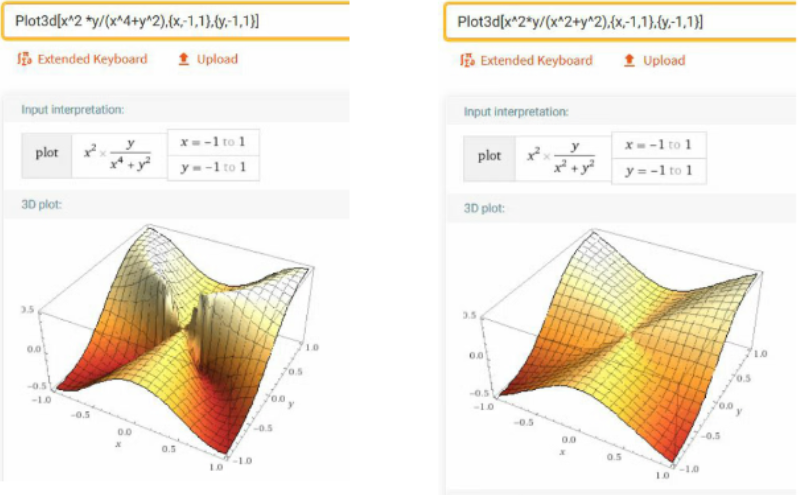
\includegraphics[width=\linewidth]{figures/contourplot_r_n_stetigkeit_beispiele}
                \caption*{Contour-Plot: Eingezeichnet werden alle \( (x,y) \), die die gegebene Gleichung erfüllen.
                Von Wolfram Alpha.}
                \label{fig:countourplot_r_n_stetigkeit_beispiele}
            \end{figure}
            \begin{figure}[H]
                \centering
                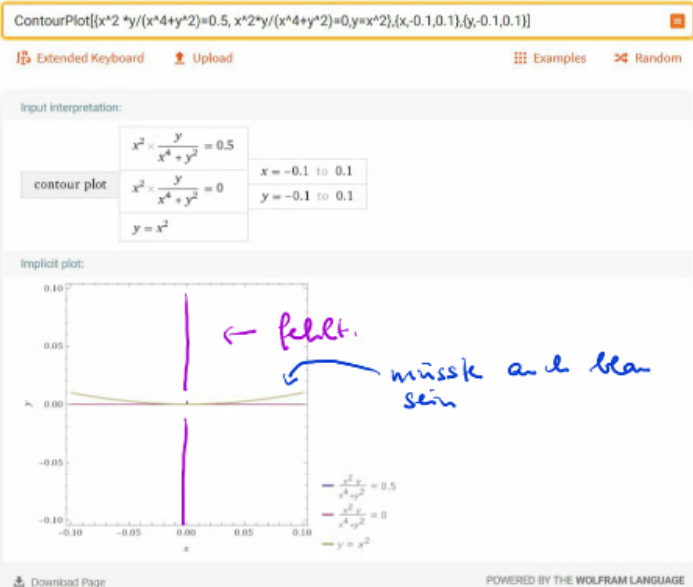
\includegraphics[width=\linewidth]{figures/contourplot_r_n_stetigkeit_beispiele_2_d}
                \label{fig:countourplot_r_n_stetigkeit_beispiele_2_d}
            \end{figure}
        \end{beispiele*}
    \end{eigenschaftenenumerate}
\end{beispiele}
\section{Vektorräume mit Skalarprodukt}
Eine spezielle Klasse von Normen sind solche, die von einem sogenannten Skalarprodukt induziert werden.
\begin{definition}\index{Skalarprodukt}
    Sei \( V \) ein Vektorraum über \( \reals \).
    Ein \emph{Skalarprodukt} auf \( V \) ist eine Abbildung \( \scalarproduct{\cdot}{\cdot}\maps V\times V\to \reals \) mit
    \begin{eigenschaftenenumerate}
        \item \label{skalarprodukt:linear}Linear: \begin{align*}
            \scalarproduct{\lambda x+\mu y}{z}=\lambda\scalarproduct{x}{z}+\mu\scalarproduct{y}{z}\quad \forall x,y,z\in V,\logicspace \lambda,\mu\in \reals
        \end{align*}
        \item \label{skalarprodukt:symmetrisch}Symmetrisch: \begin{align*}
            \scalarproduct{x}{y}=\scalarproduct{y}{x} \forall x,y\in V
        \end{align*}
        \item \label{skalarprodukt:positiv_definit}Positiv definit: \begin{align*}
            \scalarproduct{x}{x}\geq 0 \text{ und } \scalarproduct{x}{x}=0\iff x=0. 
        \end{align*}
    \end{eigenschaftenenumerate}
    
\end{definition}
\begin{bemerkung*}
    Mit \ref{skalarprodukt:symmetrisch} folgt auch die Linearität im zweiten Argument.
\end{bemerkung*}
\begin{beispiele*}
    \begin{itemize}
        \item \( \reals^n \), \( \scalarproduct{x}{y}=\sum_{i=1}^{n}x_i y_i \): Euklidisches Skalarprodukt.
        \begin{figure}[H]
            \centering
            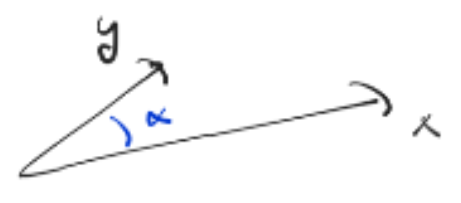
\includegraphics[width=0.3\linewidth]{figures/euklidisches_skalarprodukt_interpretation}
            \caption*{interpretation}
            \label{fig:euklidisches_skalarprodukt_interpretation}
        \end{figure}
        \( Y \) geht durch Drehstreckung aus \( x\neq 0 \) hervor:
        \begin{align*}
            y=\norm{y}_{\text{E}} \begin{pNiceMatrix} \Cos{\alpha} & -\Sin{\alpha}\\ \Sin{\alpha}& \Cos{\alpha} \end{pNiceMatrix} \frac{x}{\norm{x}_{\text{E}}}.
        \end{align*}
        Dann gilt:
        \begin{align*}
            \scalarproduct{x}{y}\begin{aligned}[t]
                &=\frac{\norm{y}_{\text{E}}}{\norm{x}_{\text{E}}}\scalarproduct{x}{\begin{pNiceMatrix} \Cos{\alpha} x_1-\Sin{\alpha}x_2 \\ \Sin{\alpha}x_1+\Cos{\alpha} x_2 \end{pNiceMatrix}}\\
                &=\frac{\norm{y}_{\text{E}}}(x_1^2\Cos{\alpha}-\cancel{x_1 x_2\Sin{\alpha}}+\cancel{x_1 x_2\Sin{\alpha}+x_2^2\Cos{\alpha}})\\
                &=\norm{y}_{\text{E}}\cdot\norm{x}{\text{E}}\cdot \Cos{\alpha}.
            \end{aligned}            
        \end{align*}
        Das Skalarprodukt misst die Projektion von \( y \) auf \( x \)
        \begin{figure}[H]
            \centering
            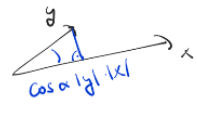
\includegraphics[width=0.3\linewidth]{figures/skalarprodukt_projektion_y_auf_x}
            \label{fig:skalarprodukt_projektion_y_auf_x}
        \end{figure}
        und umgekehrt
        \begin{figure}[H]
            \centering
            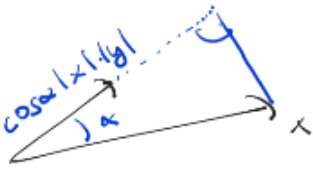
\includegraphics[width=0.3\linewidth]{figures/skalarprodukt_projektion_x_auf_y}
            \label{fig:skalarprodukt_projektion_x_auf_y}
        \end{figure}
        \item \( \reals^n \) mit \( \scalarproduct{x}{y}_W=\sum_{i=1}^{n}w_i x_i y_i \), \( w=(w_1,\dotsc, w_n) \) Gewichtsvektor, \( w_i>0 \).
        \item \( \reals^2 \) mit \( \scalarproduct{x}{y}\definedas 2x_1y_1-x_1y_2-x_2y_1+2x_2y_2 \) (zu überprüfen ist die Positive Definitheit).
        \item \emph{Kein} Skalarprodukt ist das Minkowski-Produkt: \( \reals^{n+1} \) mit \( ((x,y))\definedas x_0y_0-\sum_{i=1}^{n}x_i y_i \).

        Denn \( ((x,x))=0\iff x_0=\pm \norm{\underline{x}}_{\text{E}} \), \( x=(x_1,\dotsc,x_n) \).
        \item \( \stetigefunktionen(\interval{a}{b}) \) mit \( \scalarproduct{f}{g}=\Integrate{f(t)g(t)}{d,a,b} \).
    \end{itemize}
\end{beispiele*}
\begin{lemma}
    Sei \( V \) VR mit Skalarprodukt \( \scalarproduct{\cdot}{\cdot} \).
    Dann ist durch \( \norm{x}\definedas\sqrt{\scalarproduct{x}{x}} \) eine Norm auf \( V \) definiert.
\end{lemma}
\begin{proof}
    \begin{proofdescription}
        \item[\ref{norm:positiv_definit}] \( \norm{x=0}  \)\timplies \( \scalarproduct{x}{x}=0 \) \( \underset{\ref{skalarprodukt:positiv_definit}}{\implies} \), \( \norm{0}=0 \) \checkmark.
        \item[\ref{norm:betrags_homogen}] \( \norm{\lambda x}=\sqrt{\lambda^2\scalarproduct{x}{x}}=\abs{\lambda}\sqrt{\scalarproduct{x}{x}} \) \tforall \( \lambda\in \reals \), \( x\in V \).
        \item[\ref{norm:dreiecksungleichung}] 
        \begin{align*}
            \norm{x+y}^2 \begin{aligned}[t]
                &=\scalarproduct{x+y}{x+y}\\
                &=\norm{x}^2+2\scalarproduct{x}{y}+\norm{y}^2\\
                &\leq \norm{x}^2+2\abs{\scalarproduct{x}{y}}+\norm{y}^2\\
                &\explain{\text{siehe \eqref{eq:cauchy_schwarzsche_ungeleichung} unten}}{\leq} (\norm{x}+\norm{y})^2\implies \triangle,
            \end{aligned}            
        \end{align*}
        denn die Wurzel ist monoton wachsend.

        Es gilt die \emph{Cauchy-Schwarzsche} Ungleichung:
        \begin{align*}
            \tag{\(*\)}\label{eq:cauchy_schwarzsche_ungeleichung} \abs{\scalarproduct{x}{y}}\leq \norm{x}\cdot \norm{y}.
        \end{align*}
        \begin{subproof}
            \begin{align*}
                0\leq \scalarproduct{x-\lambda y}{x-\lambda y}=\norm{x}^2-2\lambda \scalarproduct{x}{y}+\lambda^2 \norm{y}^2\quad \forall x,y\in V\logicspace \lambda\in\reals,
            \end{align*}
            also speziell für \( y\neq 0 \) (für \( y=0 \) gilt die Ungleichung sowieso) und \( \lambda=\frac{\scalarproduct{x}{y}}{\norm{y}^2} \):
            \begin{align*}
                0\leq \norm{x}^2-\frac{\scalarproduct{x}{y}^2}{\norm{y}^2}.
            \end{align*}
        \end{subproof}
    \end{proofdescription}
\end{proof}
Einen Vektorraum mit Skalarprodukt betrachten wir immer als mit der von Skalarprodukt induzierten Norm, also Metrik, also Topologie.

Nicht jede Norm wird von einem Skalarprodukt induziert. Es gilt
\begin{lemma}
    Sei \( (V,\norm{\cdot}) \) normierter VR\@ Dann wird \( \norm{\cdot} \) von einem Skalarprodukt induziert genau dann, wenn die Parallelogramm-Gleichung gilt:
    \begin{align*}
        \norm{x+y}^2-\norm{x-y}^2=2(\norm{x}^2+\norm{y}^2)\quad \forall x,y\in V.
    \end{align*}
    \begin{figure}[H]
        \centering
        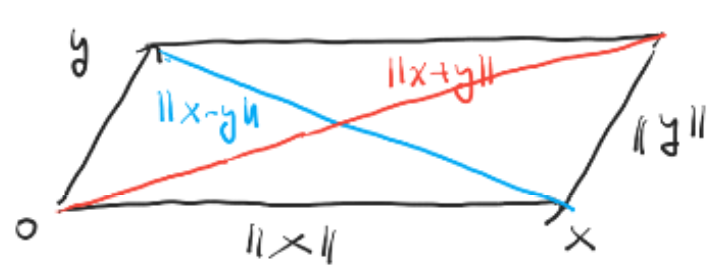
\includegraphics[width=0.5\linewidth]{figures/parallelogramm_gleichung_namenserklaerung}
        \caption*{Erklärung für den Namen. \( \reals^2 \), \( \norm{\cdot}=\norm{\cdot}_{\text{E}} \).}
        \label{fig:parallelogramm_gleichung_namenserklaerung}
    \end{figure}    
\end{lemma}
\begin{proof}
    \begin{proofdescription}
        \item[\hin] Sei \( \norm{x}=\sqrt{\scalarproduct{x}{x}} \). Dann gilt
        \begin{align*}
            \norm{x+y}^2+\norm{x-y}^2 \begin{aligned}[t]
                &=\scalarproduct{x+y}{x+y}+\scalarproduct{x-y}{x-y}\\
                &=2\norm{x^2}+0+2\norm{y^2}.
            \end{aligned}
        \end{align*}
        \item[\rueck] Erfülle \( \norm{\cdot} \) die Parallelogramm-Gleichung.
        \begin{behauptung*}
            Durch \enquote{Polarisation}, also
            \begin{align*}
                \scalarproduct{x}{y}\definedas \frac{1}{4}(\norm{x+y}^2-\norm{x-y}^2)
            \end{align*}
            ist ein Skalarprodukt definiert mit \( \norm{x}=\sqrt{\scalarproduct{x}{x}} \).
        \end{behauptung*}
        \begin{subproof}
            \begin{proofdescription}
                \item[2.\@ \Beh:] \( \scalarproduct{x}{x}=\frac{1}{4}\norm{2x}^2 \) \checkmark.
                \item[1.\@ \Beh:] \begin{itemize}
                    \item Aus der 2.\@ \Beh folgt die positive Definitheit aus der Nichtausgeartetheit und Positivität der Norm.
                    \item Die Symmetrie folgt sofort aus der Definition.
                    \item Linearität. Wir zeigen zunächst Additivität:
                    \begin{enumerate}[label=\rechtsklammer{\arabic*}]
                        \item \( \scalarproduct{x+u}{y}+\scalarproduct{x-u}{y}=\scalarproduct{x}{y} \)
                        \begin{subproof}[denn:]
                            \begin{align*}
                                \text{linke Seite}\begin{aligned}[t]
                                    &=\frac{1}{4}(\begin{aligned}[t]
                                        &\norm{x+u+y}^2-\norm{x+u-y}^2\\
                                        &+\norm{x-u+y}^2-\norm{x-u-y}^2
                                    \end{aligned}
                                    )\\
                                    &\explain{\text{Parallelogramm-Gleichung}}{=}\frac{1}{2}(\norm{x+y}^2+\norm{u}^2-\norm{x-y}^2-\norm{u}^2)\\
                                    &=\frac{1}{2}(\scalarproduct{x+y}{x+y}-\scalarproduct{x-y}{x-y})\\
                                    &=2\scalarproduct{x}{y}.
                                \end{aligned}
                            \end{align*}
                        \end{subproof}
                        Damit auch gleich gezeigt:
                        \item \label{norm_hat_skalarprodukt:beweis:zwei_multiplikativitaet}\( \scalarproduct{2x}{y}=2\scalarproduct{x}{y} \) (setze \( u=x \)) und mit \( x=u+v \), \( y=u-v \) folgt
                        \item \label{norm_hat_skalarprodukt:beweis:additivitaet}Additivität:
                        \begin{align*}
                            \scalarproduct{x}{y}+\scalarproduct{y}{z}\begin{aligned}[t]
                                &=\scalarproduct{u+v}{z}+\scalarproduct{u-v}{z}\\
                                &=2\scalarproduct{u}{z}\\
                                &\underset{\ref{norm_hat_skalarprodukt:beweis:zwei_multiplikativitaet}}{=}\scalarproduct{2u}{z}\\
                                &=\scalarproduct{x+y}{z}
                            \end{aligned}
                        \end{align*}
                        \item \label{norm_hat_skalarprodukt:beweis:natuerliche_multiplikativitaet}per Induktion \( \scalarproduct{nx}{y}=n\scalarproduct{x}{y} \) \tforall \( n\in \naturals \), denn
                        \begin{align*}
                            \scalarproduct{(n+1)x}{y}\begin{aligned}[t]
                                &=\scalarproduct{nx+x}{y}\\
                                &\overset{\ref{norm_hat_skalarprodukt:beweis:additivitaet}}{=}\scalarproduct{nx}{y}+\scalarproduct{x}{y}\\
                                &\overset{\text{IV}}{=}n\scalarproduct{x}{y}+\scalarproduct{x}{y}\\
                                &=(n+1)\scalarproduct{x}{y}.
                            \end{aligned}
                        \end{align*}
                        \item \label{norm_hat_skalarprodukt:beweis:negativ_natuerliche_multiplikativitaet} Für \( \lambda\in -\naturals_0 \) gilt
                        \begin{align*}
                            \lambda\scalarproduct{x}{y}-\scalarproduct{\lambda x}{y}\begin{aligned}[t]
                                &=\lambda\scalarproduct{x}{y}-\scalarproduct{\abs{\lambda}(-x)}{y}\\
                                &=\lambda\scalarproduct{x}{y}-\abs{\lambda}\scalarproduct{-x}{y}\\
                                &=\lambda(\scalarproduct{x}{y}+\scalarproduct{-x}{y})\\
                                &=0
                            \end{aligned}
                        \end{align*}
                        \item Für \( \lambda\in \rationals \), \( \lambda=\quot{m}{n} \), \( m,n\in \wholes \):
                        \begin{align*}
                            n\scalarproduct{\frac{m}{n}x}{y}\underset{\ref{norm_hat_skalarprodukt:beweis:natuerliche_multiplikativitaet},\ref{norm_hat_skalarprodukt:beweis:negativ_natuerliche_multiplikativitaet}}{=}\scalarproduct{mx}{y}=m\scalarproduct{x}{y}.
                        \end{align*}
                        \item Für \( \lambda\in \reals \) existiert \( (\lambda_n)_n\subset \rationals \), \( \lambda_n\goesto \lambda \). Da \( \norm{\cdot} \) stetig ist, so auch \( \scalarproduct{\cdot}{\cdot} \)
                        \begin{align*}
                            \scalarproduct{\lambda x}{y}\begin{aligned}[t]
                                &=\scalarproduct{\lim \lambda_n x}{y}\\
                                &=\lim \scalarproduct{\lambda_n x}{y}\\
                                &=\lim \lambda_n \scalarproduct{x}{y}\\
                                &=\lambda\scalarproduct{x}{y}.
                            \end{aligned}
                        \end{align*}
                        Symmetrie \timplies es genügt, das erste Argument zu untersuchen.
                    \end{enumerate}
                \end{itemize} 
            \end{proofdescription}
        \end{subproof}
    \end{proofdescription}
\end{proof}
\begin{beispiel*}
    \( \norm{\cdot}_{\text{max}} \) wird nicht von einem Skalarprodukt induziert: Sei \( x=e_1\), \( y=e_2 \). Dann gilt:
    \begin{align*}
        \norm{e_1+e_2}^2_{\text{max}}+\norm{e_1-e_2}^2_{\text{max}}=1+1=2,
    \end{align*}
    aber
    \begin{align*}
        2(\norm{e_1}^2_{\text{max}}+\norm{e_2}^2_{\text{max}})=4.
    \end{align*}
\end{beispiel*}
